\documentclass[preview]{standalone}
\usepackage[utf8]{inputenc}

\usepackage{tikz}


\begin{document}


\tikzset{every picture/.style={line width=0.75pt}} %set default line width to 0.75pt        

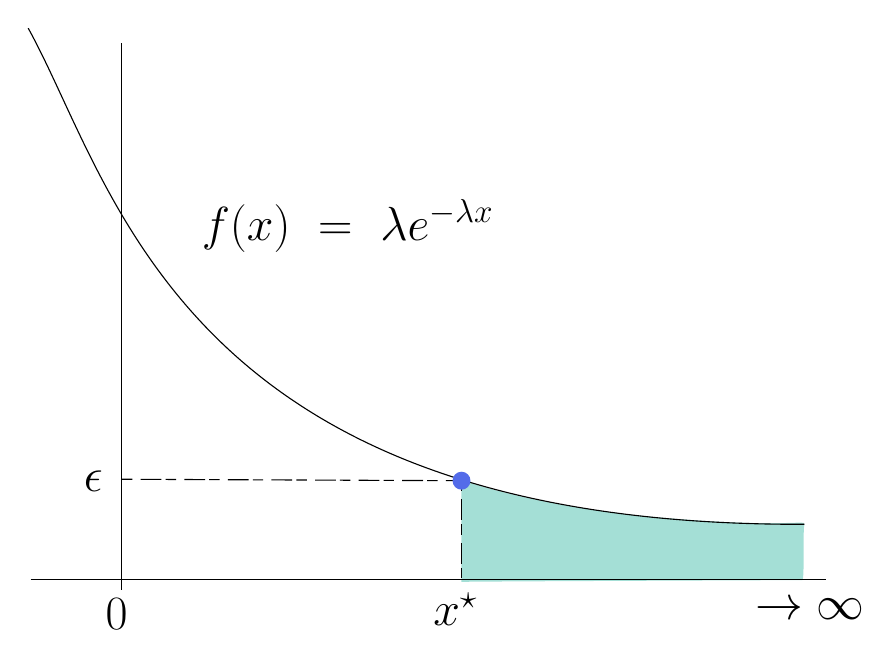
\begin{tikzpicture}[x=0.75pt,y=0.75pt,yscale=-1,xscale=1]
%uncomment if require: \path (0,310); %set diagram left start at 0, and has height of 310

%Shape: Polygon Curved [id:ds7552742596700892] 
\draw  [draw opacity=0][fill={rgb, 255:red, 164; green, 223; blue, 214 }  ,fill opacity=1 ] (264,218.25) .. controls (264.01,217.51) and (295.59,230.15) .. (357.19,235.75) .. controls (418.79,241.35) and (430.2,236.84) .. (429.25,239.25) .. controls (428.3,241.66) and (429.42,266.13) .. (428.17,266.13) .. controls (426.92,266.13) and (264.2,266.79) .. (264,267) .. controls (263.8,267.21) and (263.99,218.99) .. (264,218.25) -- cycle ;
%Straight Lines [id:da17795005541509068] 
\draw    (100,7.55) -- (100,270.88) ;
%Straight Lines [id:da6636214169523407] 
\draw    (56.45,266) -- (99.5,266) -- (439.45,266) ;
%Straight Lines [id:da012497994863657547] 
\draw  [dash pattern={on 3.75pt off 3pt on 7.5pt off 1.5pt}]  (100.45,217.55) -- (264,218.25) ;
%Straight Lines [id:da8193622880586044] 
\draw  [dash pattern={on 3.75pt off 3pt on 7.5pt off 1.5pt}]  (264,218.25) -- (264,267) ;
%Curve Lines [id:da09255024557876801] 
\draw    (55.25,0.25) .. controls (97.25,76.25) and (128.25,240.25) .. (429.25,239.25) ;
%Shape: Circle [id:dp6651207261324645] 
\draw  [draw opacity=0][fill={rgb, 255:red, 83; green, 107; blue, 233 }  ,fill opacity=1 ] (259.68,218.25) .. controls (259.68,215.87) and (261.62,213.93) .. (264,213.93) .. controls (266.38,213.93) and (268.32,215.87) .. (268.32,218.25) .. controls (268.32,220.63) and (266.38,222.57) .. (264,222.57) .. controls (261.62,222.57) and (259.68,220.63) .. (259.68,218.25) -- cycle ;

% Text Node
\draw (80.8,212.4) node [anchor=north west][inner sep=0.75pt]  [font=\LARGE]  {$\epsilon $};
% Text Node
\draw (137.6,81.6) node [anchor=north west][inner sep=0.75pt]  [font=\LARGE]  {$f( x) \ =\ \lambda e^{-\lambda x}$};
% Text Node
\draw (249.2,270.9) node [anchor=north west][inner sep=0.75pt]  [font=\LARGE]  {$x^{\star }$};
% Text Node
\draw (404.34,273.73) node [anchor=north west][inner sep=0.75pt]  [font=\LARGE]  {$\rightarrow \infty $};
% Text Node
\draw (91.3,273.98) node [anchor=north west][inner sep=0.75pt]  [font=\LARGE]  {$0$};


\end{tikzpicture}


\end{document}

